%! TEX root=./master.tex

\lecture{3}{2020-09-22}{}

\paragraph{Operators}
Operators and their precedense.

\includegraphics[width=0.8\textwidth]{03_01_operators.png}

Operators \code{=} are right-to-left while general arithmetic operators are left-to-right associative.

Assignments are expressions in C, whereas they are statements in most other languages.

\paragraph{Casting}
Is a prefix operator which takes a value of a particulare type and casts it to another, designated value. The bit-representation does usually not change, but sometimes it does.

\paragraph{Arrays}
An array is a finite vector of values of the same type. C does not check array bounds. There are certain compilers which check this but we should not assume that.

Declaration with \code{float data[5];}. We do not know that the initial value is. The easiest way is to assign \code{= \{\};} and this should always be done!\\
Assignment is done one-by-one or directly as \code{= \{1, 2, 3\}} and access is via \code{data[0]}.

Multidimensional arrays are stored in row-major in a continuous array. Meaning they are stored as $a[0][0], \dots, a[1][0], \dots, a[2][0], \dots, a[2][2]$.

It is not possible to figure out the length of the array.

\paragraph{Strings}
Strings are an array of chars. The end of the array is marked by the null character $\\0$. We could assing it directly as an array of chars \code{= \{'a', 'b', '\\0'\}} (we must add the null character), but it is easier to directly assign the sting as \code{= "ab"}.

There are no built-in methods for manipulating strings, but there are many libraries which support this. For example \code{<string.h>} is such a library and their manipulation methods have the format \code{strxxx()}.

\subsubsection{Integers}

\paragraph{Represent Integers}
As a sequence of bytes. x86 uses little-endian meaning that the least significant byte comes first.

\paragraph{Bit-Level Operations}
Manipulate single bits.

\begin{tabular}{c | c}
    $\&$ & and\\
    $|$ & or\\
    $\tilde{}$ & not\\
    $\hat{}$ & xor
\end{tabular}

We can also use the to represent and manipulate sets. We encode bit vectors in a certain way.

\paragraph{Logical Operators}
Viewing data as true and false.

\begin{tabular}{c | c}
    $\&\&$ & and\\
    $||$ & or\\
    $!$ & not
\end{tabular}

\paragraph{Shift Operations}
\begin{itemize}
    \item Left shift: $x << y$ shifts bit-vector $x$ left $y$ positions
        \begin{itemize}
            \item Fill right with $0$s.
        \end{itemize}
    \item Right shift: $x >> y$ shift bit-vector $x$ right $y$ positions
        \begin{itemize}
            \item Logical shift: fill with $0$s (if int is signed)
            \item Arithmetic shift: replicate most significant bit (if int is unsigned)
        \end{itemize}
\end{itemize}

\paragraph{Integer Ranges}

\begin{itemize}
    \item UMin $= 0$
    \item UMax $= 2^w -1$
    \item TMin $=-2^{w - 1}$
    \item TMax $=2^{w-1} - 1$
\end{itemize}

\code{<limits.h>} provides \code{ULONG_MAX}, \code{LONG_MAX}, \code{LONG_MIN}...

\paragraph{Conversation}

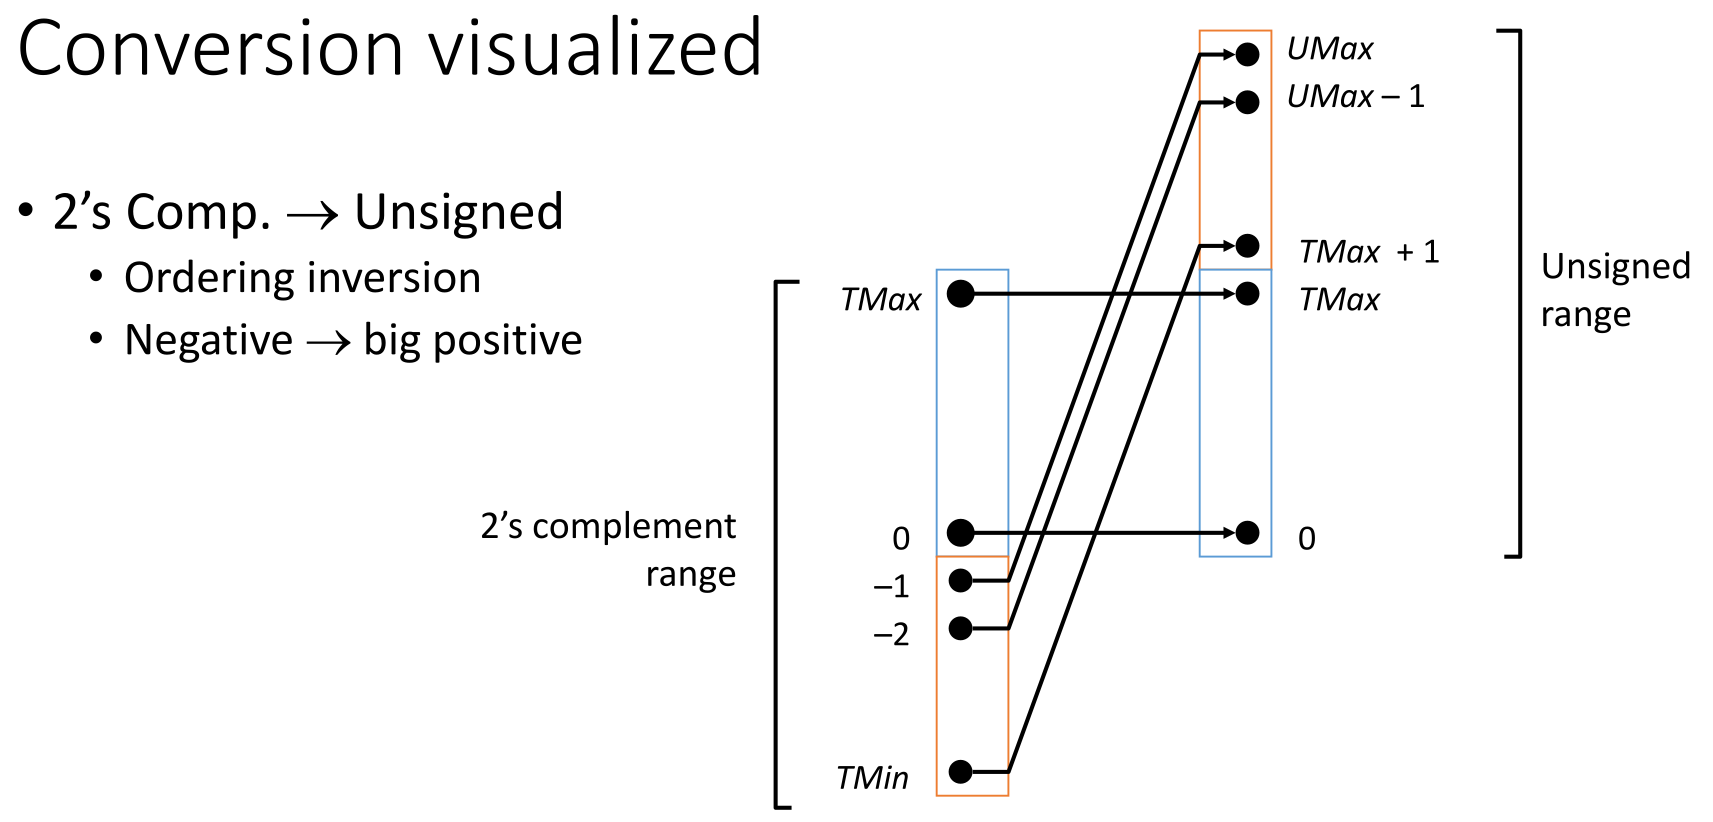
\includegraphics[width=0.8\textwidth]{03_01_conversation.png}

\paragraph{Signed vs Unsigned}
Default is considered as signed, unsigned hat \code{U} prefix. We can explicitly and implicitly cast between unsigned and signed numbers.

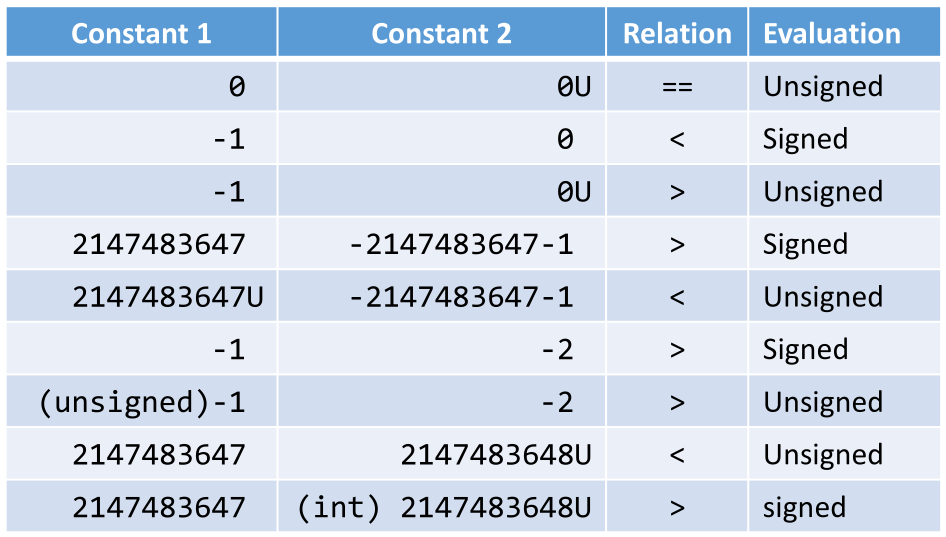
\includegraphics[width=0.8\textwidth]{03_02_numbercasting.png}

When signed and unsigned are mixed in an expression, the signed values are implicitly cast to unsigned. This included comparison operators.
